\documentclass[a4paper,addpoints,12pt]{exam}
%\documentclass[a4paper,answers,addpoints,12pt]{exam}
\unframedsolutions

%entorno para química: texto y math mode
%\newcommand*\chem[1]{\textup{#1}}
\newcommand*\chem[1]{\ensuremath{\mathrm{#1}}}

%tamaños fuentes extra: 8,9,14,17,20
	\usepackage{extsizes}

\usepackage[dvipsnames]{xcolor}
\usepackage{array,amsmath,fancybox,amsfonts,graphicx,amssymb,wasysym,latexsym,slashed,subfigure,calc}
%símbolo bonito para qed
\usepackage{amsthm}
	%\newcommand{\mc}[3]{\multicolumn{#1}{#2}{#3}}
\newcommand{\halmos}{\vspace*{-4mm}
	
					\begin{flushright}
						\rule{1mm}{2.5mm} 
					\end{flushright}\vspace*{-8mm}
						
					  }
\renewcommand{\qed}{\halmos}

\usepackage{pdfpages}


\usepackage{mdframed}

%caja bonita
  \usepackage[many]{tcolorbox}
\definecolor{titlebg}{RGB}{80,100,72}
\newtcolorbox{learn}{
  breakable,
  enhanced,
  arc=0pt,
  outer arc=0pt,
  colframe=titlebg,
  colback=titlebg!7,
  overlay unbroken and first={
    \node[
      draw=titlebg,
      fill=titlebg,
      rotate=270,
      anchor=north west,
      text=white,
      font=\bfseries
    ]
    at (frame.north east)  
    {DATOS};
  }
}

\usepackage{anysize}
	%\marginsize{left}{right}{top}{bottom}
    \marginsize{.55cm}{.4cm}{.7cm}{.5cm}
    
\usepackage[spanish]{babel}
\usepackage[utf8]{inputenc}

\usepackage{sidecap}
\usepackage{mwe,float}

%redefiniciones
\pointpoints{punto}{puntos}
\bonuspointpoints{punto}{puntos}
\hqword{Pregunta} %substitutes text for \Question"
%\vpgword{Pág.}%substitutestext for \Page"
\hpword{Máx.}%substitutes text for \Points"
\hsword{Nota}%substitutes text for \Score"
\htword{Total}%substitutes text for \Total:"

\chqword{Pregunta}
\chpword{Máx.}
\chsword{Nota}
\chtword{Total}
\chbpword{Puntos \textit{bonus}}

\renewcommand{\solutiontitle}{\noindent\textbf{Solución:}\par\noindent}



%versores: %uso: \uveci\ne\hat{\imath}_{\uvec{i}}+\uvec{j}+\uvec{k}$
	\usepackage{bm}
	\newcommand{\uveci}{{\bm{\hat{\textnormal{\bfseries\i}}}}}
	\newcommand{\uvecj}{{\bm{\hat{\textnormal{\bfseries\j}}}}}
	\DeclareRobustCommand{\uvec}[1]{{%
 	 \ifcsname uvec#1\endcsname
  	   \csname uvec#1\endcsname
  	 \else
   		 \bm{\hat{\mathbf{#1}}}%
   		\fi
									}}

%fuentes
%	\usepackage[T1]{fontenc}
%	\usepackage{fourier}


\usepackage[T1]{fontenc}
\usepackage{mathpazo}

	%\usepackage[T1]{fontenc}
	\usepackage{librebaskerville}

\usepackage{amssymb,amsmath}
\usepackage{graphicx,graphics}
\usepackage{color}
	%	\colorgrids %grids con color
	%	\definecolor{GridColor}{gray}{0.8}
		%grid
%			\setlength{\gridsize}{5mm}
%   			 \setlength{\gridlinewidth}{0.1pt}

%fracciones en texto más elaboradas
	\usepackage{xfrac}

%mejora en la exposición de guarismos
	\usepackage{numprint}
 
%caption
\usepackage[font=small,labelfont=bf,
labelsep=endash]{caption}
	
%soluciones sombreadas	
\shadedsolutions


\checkboxchar{$\Box$}
\checkedchar{$\blacksquare$}

\usepackage{everypage,draftwatermark} %Marca de agua
\SetWatermarkText{Xtra}
\SetWatermarkScale{2}
\SetWatermarkLightness{0.95}



\pagestyle{headandfoot}
%\runningheadrule
%\firstpageheader{Física para Biólogos}{Boletín 1a}{1 de octubre de 2011}
%\runningheader{Física para Biólogos}
%              {Boletín 1a, Página \thepage\ de \numpages}
%            {1 de octubre de 2011}
%\firstpagefooter{}{}{}
%\runningfooter{}{}{}


\header{%\includegraphics[scale=.25]{iesgd2.jpeg} 
		\hspace*{.5cm}\vspace*{-.4cm}
		
\includegraphics[scale=.35]{a.jpeg}}       
      {%\\Noviembre de 2019
       }
       {\large \textit{Extra}\textbf{B2}}
       %aleph, beth, gimel, daleth
       
%pie de página

   %enumera en todas menos en la primera
   %\runningfootrule

  % enumera en todas
  % \footrule
   \footer{}{}{}
   %\footer{}{Página \thepage\ de \numpages}{\iflastpage{}}
   
%%página blanco
%\usepackage{afterpage}
%%uso \afterpage{\blankpage}
%
%\newcommand\blankpage{%
%    \null
%    \thispagestyle{empty}%
%    \addtocounter{page}{0}%
%    \newpage}



%
%%indents en questions
%
\renewcommand{\questionshook}{%
  \setlength{\leftmargin}{3ex}%
    \setlength{\rightmargin}{2ex}
%  \setlength{\labelsep}{5pt}
%  \setlength{\labelwidth}{0pt}%
}
%%
%\renewcommand{\partshook}{%
%  \setlength{\leftmargin}{3ex}%
%  \setlength{\rightmargin}{2ex}
%  \setlength{\labelsep}{1ex}
%  \setlength{\labelwidth}{0pt}%
%  \def\makelabel##1{##1}%
%}


\begin{document}
\begin{coverpages}
%\pagenumbering{gobble}
%formato de preguntas
\qformat{\textbf{Pregunta \thequestion}\quad (\thepoints)\hfill}

\thispagestyle{empty}
\vspace*{-2cm}



 {\begin{center} \Huge FÍSICA---\textit{Extra}\textbf{B2}\end{center}}
 \vspace{1cm}
 
\fbox{\parbox{17cm}{\textbf{Nombre y apellidos}:
\Large 
				}
	}
\vspace{1mm}

%\fbox{\parbox{10cm}{\textbf{Grupo, subgrupo}:
%\vspace*{10mm}
%				}
%	}


\vspace*{\fill}
	
\begin{learn}
{
\vspace{5mm}
$$\triangleright\;h\simeq 6.626\cdot 10^{-34}\;J\,s\hspace{1.1cm} \triangleright\;c_0\simeq 3\cdot 10^8\;m\,s^{-1}\hspace{1.1cm} \triangleright\;\hbar c\simeq 197\;eV\,nm$$
\vspace{-5mm}

$$\triangleright\;m_{e}c_0^2\simeq 511\;keV\hspace{1cm} 1\;eV\simeq 1.6\cdot 10^{-19}\;J$$
\vspace{-5mm}

$$\triangleright\;K\simeq 9\cdot 10^{9}\; N\, m^2\, C^{-2}\hspace{1cm}\triangleright\;G\simeq 6.67\cdot 10^{-11}\;N\,m^2\,kg^{-2}$$
\vspace{-7mm}

$$\triangleright\; M_{\text{Júpiter}}\simeq 1.9\cdot 10^{27}\;kg\hspace{1cm}
\triangleright\;R_{\text{Júpiter}}\simeq 69\, 911\;km\hspace{1cm} \triangleright\;m_{\text{Juno}}\simeq 3\,625\;kg	$$			
 }
\end{learn}
\end{coverpages}


\newpage
\vspace*{-3ex}

\begin{questions}
	
	\begin{question}[2]
	
	 Desde el día 5 de julio de 2016 la sonda \textit{Juno} describe una órbita polar alrededor de \textit{Júpiter} con objeto de estudiar características atmosféricas y estructurales del gigante gaseoso. Suponiendo que la órbita sea circular y sabiendo que su altura sobre el planeta es de $4\,300\;km$:
		\begin{parts}
			\part Calcula la \textbf{energía cinética} de \textit{Juno} y su periodo de rotación.
			
			\part Calcula la \textbf{energía} que habría que comunicar a \textit{Juno} para que abandone el campo gravitatorio de \textit{Júpiter}.
						
		\end{parts}
		
	\qed
	\end{question}
	
	
%
%	\begin{question}[2]
%		\textbf{(Islas Canarias, Ordinaria, 2017)} Una lente convergente de un proyector de diapositivas que tiene una distancia focal de $16\;cm$ proyecta nítidamente la imagen de una diapositiva de $3\;cm$ de alto sobre una pantalla que se encuentra a $4\;m$ de la lente.
%		\begin{parts}
%			\part ¿A qué \textbf{distancia} de la lente está colocada la diapositiva y cuál es el \textbf{aumento} de la imagen formada por el proyector en la pantalla?
%			
%			\part Realiza el \textbf{diagrama de rayos} de la situación planteada.
%				
%		\end{parts}
%	\qed
%	\end{question}
	
  
	\begin{question}[2]
	\vspace{0ex}
	
		\begin{parts}
			\part Una lente convergente de un proyector de diapositivas que tiene una distancia focal de $16\;cm$ proyecta nítidamente la imagen de una diapositiva de $3\;cm$ de alto sobre una pantalla que se encuentra a $4\;m$ de la lente.  Calcula la \textbf{distancia} a la que está colocada la diapositiva desde la lente y realiza el \textbf{diagrama de rayos}.
			
			\part Determine la \textbf{masa} del ion potasio, \chem{K^+}, si al penetrar con una velocidad $v=8\cdot 10^4\; ms^{-1}$ en un campo magnético uniforme $\vec B=0.1\,\hat{k}\;T$, describe una trayectoria circular de $0.4\; m$  de radio.
			
		\end{parts}
	\qed
	\end{question}	
	
	
	
	\begin{question}[2]
	 Por una cuerda muy larga se propaga un movimiento ondulatorio caracterizado por la ecuación:
	$$y(x,t)=3\sin\left(7\pi\left[\frac{2t}{5}-\frac{x}{2}\right]\right),\hspace{.5cm}\text{\small(SI).}$$
		\begin{parts}
			\part Halla el \textbf{periodo}, la \textbf{frecuencia}, el \textbf{número de onda} y la \textbf{velocidad de propagación} de la onda armónica.
			\part Calcula la \textbf{diferencia de fase} en $\Delta t=0$ para dos puntos de la cuerda que están separados por una distancia $\sfrac{\lambda}{3}$.
			
					
		\end{parts}
	\qed
	\end{question}
	
	
	\begin{question}[2]
	 En un estadio de fútbol, el público hace \textit{la ola} para celebrar la buena actuación del equipo local. Los espectadores vuelven a levantar los brazos cada $10\;s$ y \textit{la ola} producida es tan grande que cualesquiera dos de ellos sentados en la misma fila y separados por una distancia de $40\;m$ se mueven sincrónicamente. Modelizando \textit{la ola} como una onda armónica:
		\begin{parts}
			\part  ¿Qué \textbf{tipo de polarización} presenta? Calcula su \textbf{longitud de onda}.			
			
			\part Las manos de cada espectador, al pasar \textit{la ola} y levantarse, se mueven verticalmente $1.0\;m$ desde el punto más bajo al más alto. Escribe la \textbf{ecuación de la onda} que se propaga en una misma fila asumiendo que $y(0,0)=0$.
			
					
		\end{parts}
	\qed
	\end{question}
	
	
	\begin{question}[2]
		
		\begin{parts}
			\part El polonio, $\chem{^{210}_{\;\;84}Po}$, es un emisor natural de partículas $\alpha$. Sabiendo que su periodo de semidesintegración es de $138$ días, calcula la \textbf{masa de polonio} que queda en una muestra de $10.0\;g$ después de $69$ días desde el inicio de la toma de medidas.
						\vspace{3mm}
			
			
			\part  Una fuente luminosa emite luz monocromática de longitud $550\;nm$, con una potencia de $2\;mW$. Se hace incidir la luz sobre un metal produciendo la emisión de electrones. La energía mínima de extracción de los electrones de la red metálica es de $2.10\;eV$. Calcula la \textbf{velocidad} del electrón más rápido que se emite y el \textbf{potencial de detención} necesario para anular la corriente fotoelectrónica.
							
		\end{parts}
	\qed
	\end{question}

\end{questions}

\newpage

\SetWatermarkText{}
\SetWatermarkScale{2.5}
\SetWatermarkLightness{0.9}

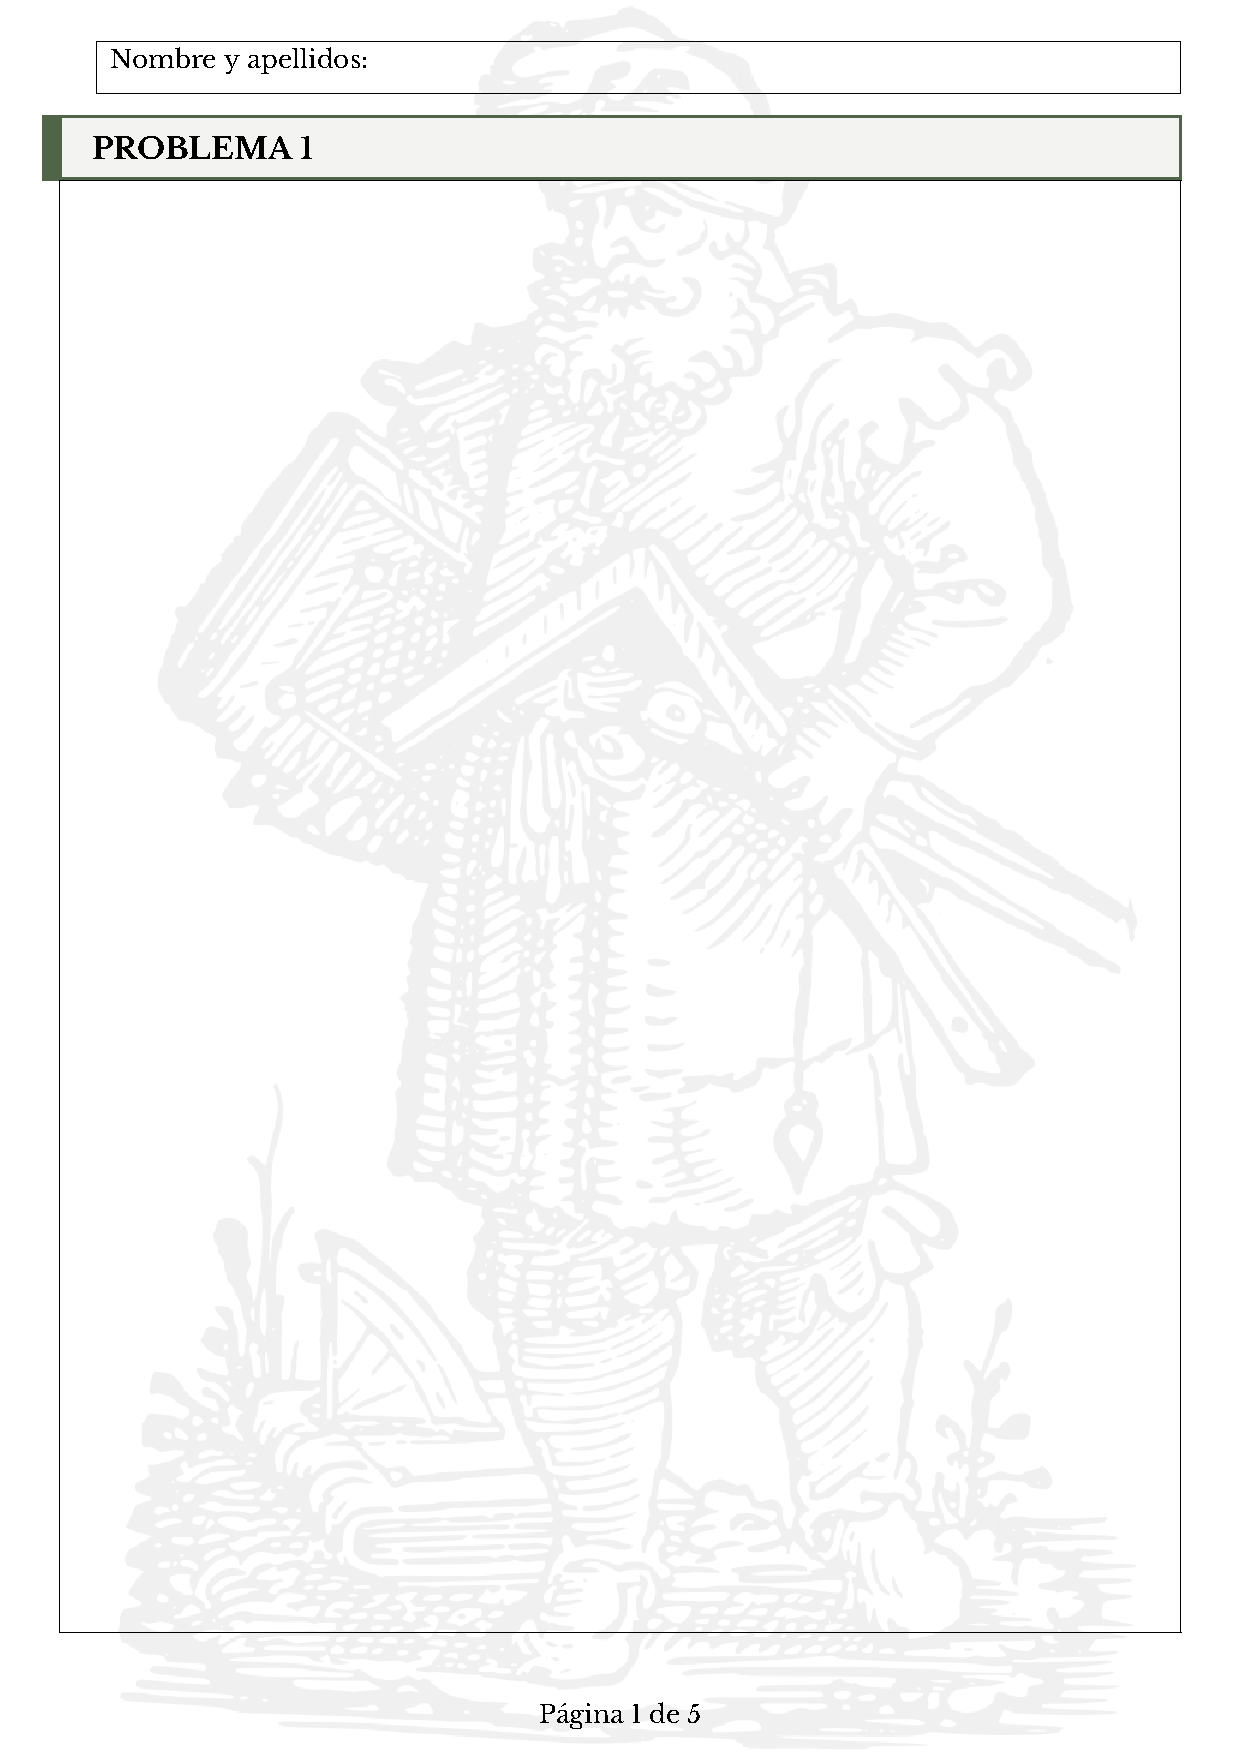
\includepdf[pages=-]{cuadernillo.pdf}

\end{document}






